\documentclass[sigconf]{acmart}

\newcommand{\FIXME}[1]{{\color{red}{\textbf{FIXME:} #1}}}
\newcommand{\amdrev}[1]{{\color{blue}{#1}}}
\newcommand{\amd}[1]{{\color{blue}{[\textbf{AMD Comment:} #1]}}}
\newcommand{\lei}[1]{{\color{cyan}{[\textbf{Lei Comment:} #1]}}}
\newcommand{\hg}[1]{{\color{green}{[\textbf{Hans Comment:} #1]}}}



\usepackage{booktabs} % For formal tables

% Copyright
%\setcopyright{none}
%\setcopyright{acmcopyright}
%\setcopyright{acmlicensed}
\setcopyright{rightsretained}
%\setcopyright{usgov}
%\setcopyright{usgovmixed}
%\setcopyright{cagov}
%\setcopyright{cagovmixed}


% DOI
\acmDOI{10.475/123_4}

% ISBN
\acmISBN{123-4567-24-567/08/06}

%Conference
\acmConference[NetCompute'18]{ACM SIGCOMM 2018 Workshop on In-Network Computing conference}{August 2018}{Budapest, Hungary} 
\acmYear{2017}
\copyrightyear{2017}

\acmPrice{15.00}

\usepackage{xspace}
\newcommand{\OurSys}{Wharf\xspace}

\usepackage{algorithm2e}
\usepackage{listings}

\begin{document}
\title{In-network computing to the rescue of faulty links}
%\title{SIG Proceedings Paper in LaTeX Format}
%\titlenote{Produces the permission block, and copyright information}
%\subtitle{Extended Abstract}

\author{Hans Giesen}
\affiliation{\institution{University of Pennsylvania}}
\author{Lei Shi}
\affiliation{\institution{University of Pennsylvania}}
\author{John Sonchack}
\affiliation{\institution{University of Pennsylvania}}
\author{Anirudh Chelluri}
\affiliation{\institution{University of Pennsylvania}}
\author{Nishanth Prabhu}
\affiliation{\institution{University of Pennsylvania}}
\author{Nik Sultana}
\affiliation{\institution{University of Pennsylvania}}
\author{Latha Kant}
\affiliation{\institution{Vencore Labs}}
\author{Anthony J McAuley}
\affiliation{\institution{Vencore Labs}}
\author{Alexander Poylisher}
\affiliation{\institution{Vencore Labs}}
\author{Andr\'e DeHon}
\affiliation{\institution{University of Pennsylvania}}
\author{Boon Thau Loo}
\affiliation{\institution{University of Pennsylvania}}

%\author{Firstname Lastname}
%\authornote{Note}
%\orcid{1234-5678-9012}
%\affiliation{%
%  \institution{Affiliation}
%  \streetaddress{Address}
%  \city{City} 
%  \state{State} 
%  \postcode{Zipcode}
%}
%\email{email@domain.com}
%
%\author{Firstname Lastname}
%\orcid{1234-5678-9012}
%\affiliation{%
%  \institution{Affiliation}
%  \streetaddress{Address}
%  \city{City} 
%  \state{State} 
%  \postcode{Zipcode}
%}
%\email{email@domain.com}
%
%\author{Firstname Lastname}
%\orcid{1234-5678-9012}
%\affiliation{%
%  \institution{Affiliation}
%}
%\email{email@domain.com}
%
%\author{Firstname Lastname}
%\orcid{1234-5678-9012}
%\affiliation{%
%  \institution{Affiliation}
%}
%\email{email@domain.com}
%
%\author{Firstname Lastname}
%\orcid{1234-5678-9012}
%\affiliation{%
%  \institution{Affiliation}
%}
%\email{email@domain.com}


% The default list of authors is too long for headers}
%\renewcommand{\shortauthors}{F. Lastname et al.}
\renewcommand{\shortauthors}{H. Giesen et al.}

\begin{abstract}
Failing network links are usually disabled, and packets are routed around them
until the links are repaired. While
it is often possible
to utilize some of a failing link's capacity, losing
what remains of a link's
capacity is typically deemed preferable to the erratic effect that unreliable links can
have on application-level behavior.

We describe a new network function that relies on in-network computing to limit
the erratic effect of failing network links, to enable the continued use of
those links until they can be repaired.
%We argue that such a network function can help mitigate rolling
%failures in datacenter networks, and that our design can interoperate
%with existing network architecture and configuration choices, such as
%for multi-path routing.

We explore the design space using ns-3, and evaluate our
implementation on a physical test-bed that includes programmable
switches and reconfigurable hardware.
Our current hardware prototype uses around 10\% of our FPGA's
resources while operating at \FIXME{30\%} of its maximum clock rate,
but can almost saturate a 10GbE link.
\hg{The current frequency of 156.25 MHz is determined by the line rate
    (=10000/64).  Higher frequencies won't benefit the throughput as the
    link will be the bottleneck.  This gives the false impression that
    a higher frequency would be better.  I would rather mention latency
    or even power consumption.}
\end{abstract}

%
% The code below should be generated by the tool at
% http://dl.acm.org/ccs.cfm
% Please copy and paste the code instead of the example below. 
%
\begin{CCSXML}
<ccs2012>
 <concept>
  <concept_id>10010520.10010553.10010562</concept_id>
  <concept_desc>Computer systems organization~Embedded systems</concept_desc>
  <concept_significance>500</concept_significance>
 </concept>
 <concept>
  <concept_id>10010520.10010575.10010755</concept_id>
  <concept_desc>Computer systems organization~Redundancy</concept_desc>
  <concept_significance>300</concept_significance>
 </concept>
 <concept>
  <concept_id>10010520.10010553.10010554</concept_id>
  <concept_desc>Computer systems organization~Robotics</concept_desc>
  <concept_significance>100</concept_significance>
 </concept>
 <concept>
  <concept_id>10003033.10003083.10003095</concept_id>
  <concept_desc>Networks~Network reliability</concept_desc>
  <concept_significance>100</concept_significance>
 </concept>
</ccs2012>  
\end{CCSXML}

\ccsdesc[500]{Computer systems organization~Embedded systems}
\ccsdesc[300]{Computer systems organization~Redundancy}
\ccsdesc{Computer systems organization~Robotics}
\ccsdesc[100]{Networks~Network reliability}

% We no longer use \terms command
%\terms{Theory}

\keywords{ACM proceedings}


\maketitle

\section{Introduction}
Advances in networking, hardware architecture, and programming
languages in recent years have converged to make the choice between
network performance and programmability easier: one can increasingly
afford both.
This has enabled research into hardware implementations of various
applications that were previously confined to software for
programmability, or to expensive and inflexible ASICs for performance.

Most prior research in this area has adapted \emph{existing}
applications to run in hardware at line rate.
Example applications include:
key-value stores~\cite{Li:2017:KHI:3132747.3132756},
network testing~\cite{Shahbaz:2013:AOS:2537857.2537880},
consensus protocols~\cite{Istvan:2016:CBI:2930611.2930639},
network stacks~\cite{Istvan:2016:CBI:2930611.2930639},
regex matching on payloads~\cite{Woods:2010:CED:1920841.1920926},
and packet filtering~\cite{Fiessler:2016:HVH:2881025.2881033}.

In this paper we describe \OurSys, which to our knowledge is the first application
of its kind. \OurSys is an in-network distributed
mitigation for faulty links.  We claim that our design requires
minimal configuration, is transparent to
end-points and does not conflict
with existing network architecture choices (e.g., the network's topology,
and how packets are routed over it). We model \OurSys using ns-3 and evaluate
implementations for CPUs and FPGAs.

\OurSys can work with various types of networks, but we think it can
be especially helpful in mitigating failing links in datacenters,
which has previously been studied by Zhuo et
al.~\cite{Zhuo:2017:UMP:3098822.3098849}.
Datacenter networks are ever more expansive and their architecture
involves a large number of links to attain a larger bisection
bandwidth. Their performance is critical to many widely-used
applications, including those running on private and public clouds.
The current practice of polling and disabling links from the edge of
the network is slow, and adds more contention over non-failing links.
\OurSys can help make such networks more resilient to failing links, with minimal configuration overhead.

Running \OurSys as an in-network function makes more sense than
running it in end-hosts since the problem that \OurSys mitigates is
scoped in the network itself. Just as some application features are
best managed end-to-end~\cite{Saltzer84end-to-endarguments}, handling
link failure seems best done at the link's level. Not only are we able to
identify the faulty link directly, but, unlike higher-layer protocols,
we can also distinguish link failure from congestion.

Programmable hardware alone is not sufficient to solve this problem: one
also needs a careful design since link management might interfere with
other features of the network, such as topology and routing~
\cite{Greenberg:2011:VSF:1897852.1897877,
NiranjanMysore:2009:PSF:1594977.1592575,
Agarwal:2014:SMS:2620728.2620758},
transport~\cite{Raiciu:2011:IDP:2043164.2018467,Alizadeh:2010:DCT:1851275.1851192}
and load balancing~\cite{Alizadeh:2014:CDC:2740070.2626316}.
In designing \OurSys we sought to make it transparent to other
features of the network, to facilitate its interoperation with
existing networks.

Our contributions include (i)~the design of \OurSys, which relies on a
link-layer forward error-correction (FEC) scheme to mitigate failing
links, and (ii)~the FPGA implementation of \OurSys to saturate 10Gbps
links. Part of our implementation is in
P4~\cite{Bosshart:2014:PPP:2656877.2656890} over SDNet, and we
transcended P4's limitations~\cite{Dang:2017:WPL:3050220.3050231} by
writing external functions in C for high-level synthesis.
They key challenge we encountered was in streaming packets through our
external functions, and we believe that our approach could be a
helpful take-away for other researchers.

The next section describes the background and related work of the problem we
are solving, before we describe our design~(\S\ref{sec:design}) and
implementation~(\S\ref{sec:implementation}), which we
evaluate~(\S\ref{sec:evaluation}) before concluding.

\begin{figure}
  \centering
  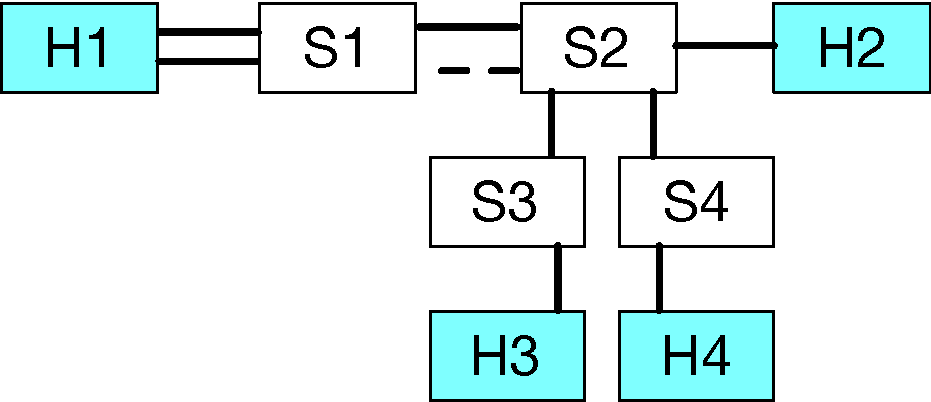
\includegraphics[width=0.3\paperwidth]{example_network.pdf}
  \caption{\label{fig:example-net}An example network consisting of four
    switches (S1-S4) and four hosts (H1-H4). Faulty links are shown as dashed lines.
    Each link is assumed to have capacity $R$ unless the link is faulty, in
    which case it has capacity $F < R$.  In this example, the failing link
    diminishes the bandwidth of H1.}
\end{figure}

\section{Background}
A communication network is architected to handle variation in its state
arising from environmental interference, component failure, congestion and
corruption of data. In this paper we describe a technique to enhance the
reliability of failing links.

Our approach could be compared to existing link-layer mitigations for
unreliable transmission, such as network-wide hop-by-hop protection, as in
X.25~\cite{X25}, and link-layer retransmission as in the 802.11~\cite{WiFi} family of
standards. The mitigation chosen for each system mostly depends on
the transmission medium: X.25 was designed to work with unreliable links,
whereas 802.11 uses a shared medium. We follow the same thinking,
and our design is based on properties of the medium: we concentrate on wired
10-Gbps Ethernet; typically such links are reliable (i.e., have low error
rates) and they are not shared (i.e., point-to-point).
Instead of using an ARQ scheme as in X.25 and 802.11, we use forward
error-correction (FEC). This simplifies our design, obviating the need for
windows and timers, and requires less memory to implement since the sender
will not attempt to resend a frame.

Our link-layer FEC complements the physical-layer FEC that is used in
high-capacity Ethernet links: the physical-layer FEC helps the link sustain a
given capacity over longer distances, whereas our FEC is intended to mitigate
a errors that do not arise because of challenging environmental factors; rather
the errors arise because of faults.

Our approach also complements higher-layer reliability measures, as provided by
TCP for example.  TCP provides end-to-end reliability, whereas we concentrate
on link-level reliability. Unlike TCP, we are able to distinguish congestion
from corruption as the cause of packet loss, and we are able to locate the
lossy links in the network. Thus we can react to them much more quickly than
TCP at the end-points. As with TCP, our mechanism results in a reduced
transmission rate, but this is necessary since the link capacity has been
reduce because of the link's failure.

\section{Design}
\label{sec:design}
%We assume that the underlying network is Ethernet, on which we implemented our
%prototype.

\OurSys infers failing links and follows a policy on how to process
frames that are about to cross failing links. It uses a \emph{forward
error-correction} scheme to enable the next hop recover frames that
were lost in transit, by using extra parity frames that are inserted
into the medium.

In this section we describe \OurSys's policy choices for managing failing
links, and how the chosen policy is followed in the network.


\subsection{Traffic classification}
\label{sec:traffic-classification}
\OurSys is configured to have a (usually small) number of traffic classes,
which partitions the frames arriving at a switch. Outbound frames are encapsulated and
complemented with parity frames, forming \emph{blocks} that are sent across
the faulty link.
Each class $c$ is defined by a map $T: c \mapsto (k, h, t)$, where $k$ is the
number of frames in a block, $h$ is the number of parity frames sent for each
block, and $t$ is the timeout.
(When the encoding timer expires, the remaining frame spaces in a block are
zeroed out to provide padding.)
The values $(k, h, t)$ influence the latency with which frames belonging to $c$
cross the switch, as well the likely recovery of frames belonging to $c$. For
example, for interactive applications we would want to use a small $k$ and $t$.

%\lei{Deleted some. Seems to be redundance of 3.3-sending proxy}
%\iffalse
%Parity frames are new frames that are put onto the medium, so by
%increasing $h$ we create more contention for the link, which reduces
%the capacity available for data from applications crossing that link.
%\fi

\subsection{Link-failure management policy}
\label{sec:policy}
For each port the policy stipulates how to react if the link becomes faulty:
  \begin{itemize}
    \item Drop frames (i.e., disable the link); or
    \item Classify the frame, encode it, and forward.
  \end{itemize}
For the latter case, the policy specifies what are the traffic classifications,
and how does each classification map into parameters $(k, h, t)$.

In principle both the map $T$ (from~\S\ref{sec:traffic-classification}) and
the policy can be decided or changed while \OurSys is running, but for
consistency not while \OurSys is actually processing frames. In practice it is
resource-efficient to engineer to a limited set of choices to support.


\subsection{Execution}
\OurSys consists of three concurrent activities carried out for each port of a
switch:
\begin{itemize}
  \item \textbf{Link monitoring agent} attempts to infer link malfunction.
  \item \textbf{Sending proxy} processes frames and adds tags before they are sent over a faulty link.
  \item \textbf{Receiving proxy} processes inbound \OurSys-tagged frames.
\end{itemize}

Frames to be sent over non-faulty links, and inbound frames that are not
\OurSys-tagged, are processed as normal by the switch. Otherwise outgoing frames
are processed by the Sending proxy prior to egress, and inbound frames by
the Receiving proxy after ingress.

\paragraph{Link monitoring agent.}
  We continuously poll network port counters to infer malfunctioning transceiver
  modules or links. This is done as in
  CorrOpt~\cite{Zhuo:2017:UMP:3098822.3098849}, but failure-inference is done
  locally on the switch, rather than remotely on a separate machine.
  Sometimes a switch cannot itself realize if one of its links is
  malfunctioning, since the malfunction would be inferable from the adjacent
  element's counters (e.g., through an increase in frame errors). Thus switches
  might need to inform each other about errors on the transmitting side. To do
  this we employ LLDP and use a custom TLV to signal to the receiving switch
  that the link (for traffic travelling in the opposite direction) is failing.
  The switch's monitoring would then follow the policy to disable the link, or
  channel outgoing frames through the Sending proxy.

\paragraph{\OurSys frame encapsulation}
Frames sent over faulty links are encapsulated as shown in Fig.~\ref{fig:format}.
The original frame is fully encapsulated, and the new header consists of the original source and destination addresses, as well as a custom EtherType for \OurSys.
After the Ethernet header we add a \OurSys tag.
%, the field-sizes of which
%are deployment-specific: the sizes we use in our implementation are specified
%in~\S\ref{sec:implementation}. \FIXME{I believe we are not specifying it}
The information in the \OurSys tag is sufficient to distinguish blocks in
non-bursty loss, as illustrated in Fig.~\ref{fig:example-loss}. If loss is
bursty then an additional small number of bits can be added to the tag to
tell blocks apart, as shown in Fig.~\ref{fig:example-loss2}.

\begin{figure}
  \centering
  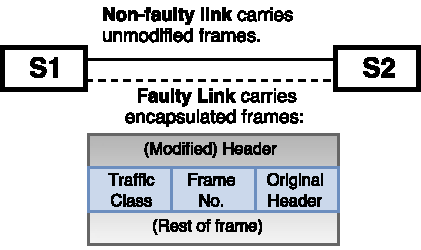
\includegraphics[width=0.25\paperwidth]{figures/paper-fig-3.pdf}
  \caption{\label{fig:format}Switches can have multiple links between them.
  Traffic on faulty links is encapsulated as shown above: the frame's EtherType
  is moved inside the \OurSys tag (and later moved back after the frame crosses
  the link), the frame's EtherType is changed to \OurSys, and the frame is
  classified to a particular Traffic Class and given a transient link-local
  identifier: these are shown as $c$ and $n$ respectively in
  Fig.~\ref{fig:example-loss}.}
\end{figure}

\begin{figure}
  \centering
  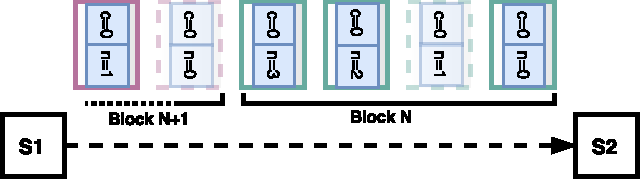
\includegraphics[width=0.35\paperwidth]{figures/paper-fig-4.pdf}
  \caption{\label{fig:example-loss}The expectation for strictly monotonic frame
  number $n$ ensures that we can distinguish successive blocks. Note that frame
  reordering is not possible because they are being sent over the same link,
  and their processing is sequential across that link.}
\end{figure}

\begin{figure}
  \centering
  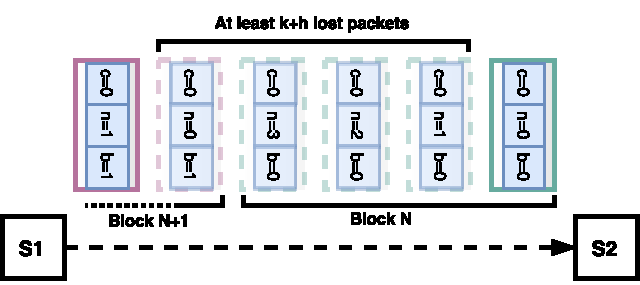
\includegraphics[width=0.35\paperwidth]{figures/paper-fig-5.pdf}
  \caption{\label{fig:example-loss2}To mitigate bursty loss, a block sequence number is added.}
\end{figure}

\paragraph{Sending proxy.}
The pseudo-code is shown in Algorithm~\ref{alg:sending}.
As with decoding, the encoding of a block (to produce parity frames) is
triggered when the block is full (all $k$ frames have been accounted for) or
$t$ for that $c$ expires (relative to when the first frame was inserted into
the block). Non-parity frames are tagged and forwarded immediately.

Due to its operation, the sending proxy can cause congestion at egress.
For example, if $k = h$, and we are receiving traffic bound for
a faulty link at rate $R$, then we would need to send at $2R$ at each interval
of $k$ incoming frames, at which time the sending proxy produces $h$ additional
frames for output. We simply drop new frames that cannot be put onto the link
fast enough (i.e., before they are placed into a block). This lack of capacity
is communicated by the $\mathit{busy}(c)$ predicate in
Algorithm~\ref{alg:sending}, which indicates that the FEC computation is
ongoing, or its results are still being serialized onto the medium. This loss
will communicate to higher-layer protocols that congestion is occurring (both
due to the link capacity being reduced, and because of the extra overhead of
sending the parity frames), and the end-hosts network stacks can react to this
congestion as they normally would.

\begin{algorithm}
\SetAlgoLined
\SetKwInOut{Input}{input}\SetKwInOut{Output}{output}
\Input{frame to be forwarded}
\Output{forwarding decision}
\uIf(\tcc*[h]{Link has been disabled}){policy = drop}{
drop frame\;
}\Else(\tcc*[h]{Use FEC}){
  $c = P(\mathrm{frame})$ \tcc*[r]{Classify the frame}
  \uIf(\tcc*[h]{Block is being sent}){busy(c)}{
drop frame\;
}\Else{
  $\overline{\mathrm{frame}}$ = encapsulate($c, \mathrm{frame}$)\;
  addToBlock($c$, $\overline{\mathrm{frame}}$)\;
  forward $\overline{\mathrm{frame}}$\;
}
}
\caption{\label{alg:sending}Sending proxy. If the block's $k$ has been reached, then addToBlock will start the process of generating and sending parity frames. This process is also began if the block's $k$ has not been reached but $t$ expires.}
\end{algorithm}

\paragraph{Receiving proxy.}
\OurSys-tagged frames are buffered as shown in Fig.~\ref{fig:example-decode},
and non-parity frames are untagged and forwarded immediately.
For each $c$, if its $t$ (relative to when the first
frame was buffered) expires, or a frame from a successive block arrives, 
then decoding is triggered. Decoding consists of using the parity frames to
reconstruct the lost data frames; if no data frames have been lost then there
is no more work to be done for this block.
%\amd{I've been assuming a simpler version...as soon as there are enough
%  packets to perform decoding, we do.  Then we discard any subsequent
%  packets that arrive in the block.  No timeout on decode.  On the FPGA
%  where we are designed for full rate when decoding, this doesn't slow
%  anything down.  On a processor that cannot maintain full-rate decoding,
%  not doing decoding could be a performance optimization.}\\
%\lei{I've switched paragraph 1 and 2, 3 and 4. This order follows the listing at the beginning,
%looks more natural to me, and avoids use-before-define. I also lifted the diagrams. It is difficult
%to understand the design from plain text for people unfamiliar with this. Also, there are too many
%details in caption of diagrams.}

%\begin{algorithm}
%\SetAlgoLined
%\SetKwFunction{FName}{addToBlock}%
%\SetKwProg{Proc}{Procedure}{\string:}{}
%\Proc{\FName{c, frame}}{
%\uIf(\tcc*[h]{Link has been disabled}){policy = drop}{
%drop frame
%}\Else(\tcc*[h]{Use FEC}){
%  $c = P(\mathrm{frame})$\;
%  addToBlock($c$, frame)\;
%}
%}
%\caption{\label{alg:sending}Adding a frame to a block for class $c$}
%\end{algorithm}
\begin{figure}
  \centering
  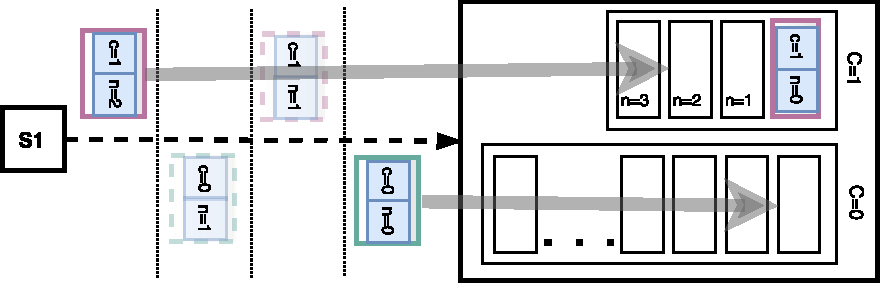
\includegraphics[width=0.4\paperwidth]{figures/paper-fig-6.pdf}
  \caption{\label{fig:example-decode}Prior to decoding each block is mapped to the buffer for its traffic class.}
\end{figure}

\section{Implementation}
\label{sec:implementation}

\newcommand{\hg}[1]{{\color{green}{[\textbf{Hans Comment:} #1]}}}

\subsection{Overview}
%To meet the performance requirements of the data center, we implemented \OurSys
We implemented \OurSys
on the Xilinx Zynq UltraScale+ MPSoC ZCU102 Evaluation Kit.  This board has 4 SFP+ cages, and we process network traffic on its
ZU9EG System-on-Chip FPGA, which consists of a quad-core ARM Cortex-A53, a
dual-core ARM Cortex-R5, and a programmable fabric with 274K lookup tables
(LUTs) and 1800 18Kb embedded memories (BRAMs).

\begin{figure}
  \centering
  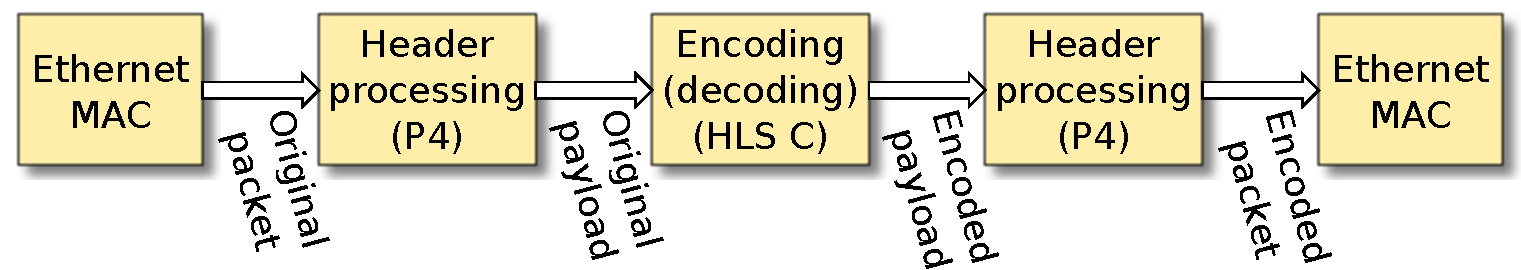
\includegraphics[width=0.4\paperwidth]{Top_level.pdf}
  \caption{\label{fig:toplevel} Block diagram of FEC encoder / decoder pipeline.
  }
\end{figure}

A top-level diagram of the implementation is shown in Fig.~\ref{fig:toplevel}.
%Packets arrive on one of the 4 SFP+ cages via a 10Gbps Ethernet cable.
%A dedicated 10~Gigabit Transceiver deserializes the packets.  After further
%processing by a dedicated Ethernet PHY and in-fabric MAC layer, the entire
%packet including Ethernet header is output on a 64-bit AXI Stream bus at 160\,MHz.
%
%The next stage in the pipeline performs packet header preprocessing.  With
%ease of implementation and portability in mind, we implemented this in P4, a
%domain-specific programming language for packet processing that is target- and
%protocol-agnostic \cite{p4_sigcomm_review2014}.
We implement header processing in
P4~\cite{Bosshart:2014:PPP:2656877.2656890}, which is compiled to FPGA
logic using Xilinx's SDNet tool suite.  Header processing (described
further in~\S\ref{sec:impl:header-processing}) includes the frame
tagging described in~\S\ref{sec:design}.

The frame is then forwarded to the FEC core, which can be an encoder (for the Sending Proxy) or decoder (for the
Receiving Proxy).
%In both cases, the FEC core
%produces payloads that are the result of, respectively, encoding or decoding
%the received group of payloads.  Similar to the header processing, the FEC core
%was also created with ease of implementation in mind.
P4 is not suitable
for
%payload processing or
exploiting the parallellism of the FEC core, so we implemented the core in
hardware-synthesizable C. The code can be compiled and executed on a
general-purpose CPU, but we can also synthesize the code for an FPGA
in Vivado HLS.  Guided by pragmas added by the developer, Vivado HLS takes
advantage of parallelism in the code to 
achieve  high performance.

The encoded or decoded output of the FEC core feeds into the header
post-processing, which encapsulates the payloads in Ethernet packets, before packets are returned to the network.

\subsection{Header processing}
\label{sec:impl:header-processing}
We use P4 to implement high-level packet processing logic and
use Xilinx's P4-SDNet toolchain to translate our P4 program into RTL
and integrate modules together.
%The translation goes through 3 steps:
%
%First, from P4 to SDNet
%
%Second, from sdnet to RTL implementaion and C++ high-level simulation
%
%Third, add preipheral blocks with Vivado Design Suit
%
Our P4 program carries out packet parsing, header tagging,
extracting payload for encoder, and
bookkeeping of packet classes.

\iffalse

what is SDNet?
intermediate language, describes the interface, layout, and data flow of data processing engines
at a level closer to RTL modules compared to P4.

\amd{not sure what value the above has -- I do suggest hoisting the SDNet
  comment into the previous section}

%introduce RTL/FPGA?

\fi

%Although P4 is easy to use and works very well in fullfilling its duty by design,
%we did meet several technical challenges in our specific task:
%
%1. P4's variables only keep their values within the processing of one packet.
%The program is stateless across packets, which makes it impossible to track
%a sequence of packets. We implement stateful logics, e.g., registers, in
%FPGA and link to P4 programs through the interface of external functions.
%This makes it possible for P4 to do bookkeeping, but also raises another problem:
%
%2. Both P4 and SDNet encourage programs working like a flow. Parser, deparser,
%variable updates and external functions are all treated as processing blocks. 
%And all blocks are chained into a Directed Acyclic Graph(DAG), starting 
%from the input port, ending in the output port. Each packet only enters
%and exits a block at most once, including the stateful registers we defined.
%This ensures the efficiency of the program, especially low latency per packet, 
%but also makes it harder to express complex logics. For example, it is forbidden
%to read a value from a register, do some calculation and then write the updated 
%value back, since the register will be accessed twice, causing a cycle.
%Updating the same register at two different branches is also forbidden to
%avoid a potential cycle.
%
%Directly designing a program following these constraints can be very messy
%and unintuitive. So we start with a more modular program that violates the
%syntax slightly and then translate it to a valid program. We think it can be 
%a future work to do the translation automatically. Currently we do this manually
%by 1)keeping in mind a dependency graph of variable updates and external function 
%calls, 2)merging concurrent calls to the same function, 3)replacing cycles with
%atomic read-modify-write functions, and 4)doing a topological sort to decide 
%the final order of code. An observation here is that most calculations used
%for tracking packets can be replace by an atomic operation "read-and-add-one",
%which makes step 3) possible.
%
%3. As is mentioned above, there is no interface designed for payload processing
%in P4. The abstract P4 provides is to see a packet as a whole. This is usually 
%tolerable for headers since they tend to be short. However, it is desirable to process
%the payload, up to nearly 1500 bytes long in Ethernet, in a cut-through way, so that we can 
%save the space for a extremely wide bus and the long latency for buffering the 
%whole packet. This lack of feature incurs some difficulties in the integration of header processor and encoder.
%Although we can literally split the system into a P4 pre-processor, a P4 post-processor, 
%and an FPGA encoder block in-between like the concept model, leaving the payload parsing task to FPGA,
%it would require considerable engineering effort and largely nullify P4's convenience.
%
%Fortunately, we found that the generated SDNet intermediate code, although not well documented,
%in fact provides the abstract of a packet stream. We are able to embed the encoder in the P4 switch by
%defining it as an external function, leaving out the actual input data. Then we 
%redirect the data stream in the generated SDNet code to include the encoder block in
%its path. In this way, the encoder is able to receive the content of the packet as a stream
%on a 64-bit wide bus, while keeping the ability to use P4 for parsing and bookkeeping.
%The modification can be finished with a script in less than 10 lines of code.
%
%\lei{well...... is this too long?}

         
Since we compute over whole frames -- and not only headers -- we could
not write our entire system in P4. In the header processing part of
our system, which is implemented in P4, we therefore sought to develop
an interface between P4 code and the more general computing we need
for FEC (described below in~\S\ref{sec:impl:fec-encoder}), which we
implement in hardware-synthesizable C.

\iffalse
The interface between P4 and external functions emerged as a very
important part of our implementation, since whole packets must flow
through it between the P4 environment to the more general logic
implementing our FEC. 
\fi
This interface emerged as a very important part of our implementaion,
since whole packets must flow through it between two different levels
of abstractions.
We found that SDNet implements an extensible
pipeline of functional blocks chained by a packet stream, to which we can add our external function. 
%This allowed us to implement our function as a stream processor, for cut-through behaviour through SDNet.
As is shown by Fig.~\ref{fig:sdnet-interface}, this allows us to implement
our function as a stream processor with cut-through behaviour and glue it
to the header processor.

\begin{figure}
  \centering
  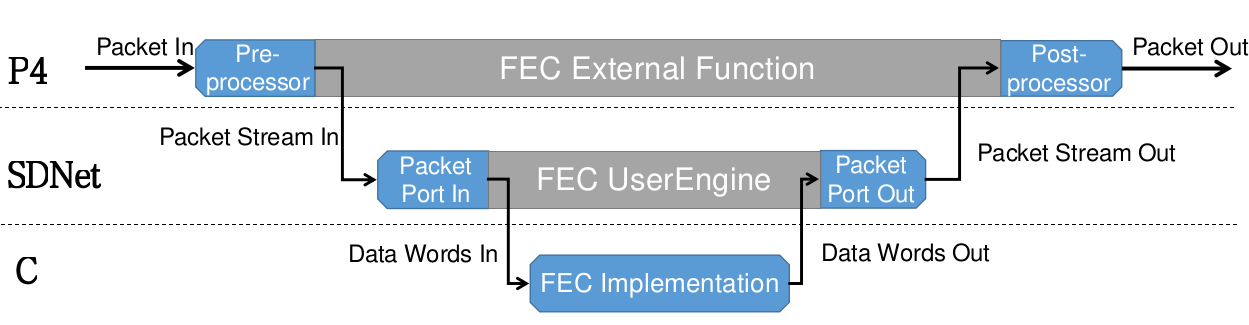
\includegraphics[width=0.4\paperwidth]{figures/sdnet-interface.png}
  \caption{\label{fig:sdnet-interface}Abstraction provided by each layer; grey blocks are translated to the pipeline illustrated in next level.}
\end{figure}

\iffalse
1. Both P4 and SDNet encourage programs working like a flow - you should never go back and touch anything
a second time. This ensures the efficiency of the program but also makes it harder to express complex
logics. We think it can be a future work to translate a loosely written program into one with such constrains.
Currently we do this manually by keeping in mind a dependency graph of program lines and doing a topological sort
to decide the final order. Using compound operations like
$read\_and\_add\_one$ also helps mitigating this problem.
\amd{I am not following this...and I doubt a reader with no knowledge of
  FPGAs or SDNet will be able to follow either.  What does ``go back'' mean
  in this context? What are you ordering? How is the read-and-add-one
  addressing the problem?}

2. P4 is designed particularly for header processing. There are many
irrelevant \amd{irrelevant is probably not the right word here} things not supported but
necessary in our work, especially payload processing. Most bookkeeping operations can be finished with the
help of external functions like $read\_and\_add\_one$, later implemented in C or Verilog. We also integrate the encoder
into the design by defining an external function for it. However, encoding payload through this interface can be a
great waste for both time and space due to P4's nature of passing and processing a packet as a whole, no matter how long it is. Fortunately, the
flexibility we seek can be found by redirecting SDNet's internal packet flow, which works similar to a 64-bit AXI Stream bus,
to the engine for encoder. This involves modification of less than 10 lines of code per SDNet program, and can be finished by a simple script.
\amd{...don't think this works for a reader either...  Yes, we want to make
the case that P4 doesn't allow payload processing (I suggest adding a note
about that above).  Do we want to dig into the fact that P4 doesn't give us
the expressiveness to stream payload processing, but SDNet does?  ... if
so, we'll need to setup the problem better here and be clearer about the
shape of the solution.}
\fi

\subsection{FEC Encoder}
\label{sec:impl:fec-encoder}

In this section we describe our generation of parity frames. Currently
we can only decode on a CPU; our FPGA implementation of the decode is
work-in-progress.

%The current implementation is limited to packet encoding, but our intention is
%to implement the decoder too.

In \OurSys, error correction is performed with a Reed-Solomon erasure (RSE) code~\cite{rse}
\hg{Note that this reference covers only error correction, not dealing with erasures}.
% Erasure codes
%require prior knowledge of which packets data is missing, as opposed to regular
%error correction codes.  This comes with the benefit of requiring fewer error
%correction bits.  RSE is a linear code, which means that every codeword can be
%obtained by a linear combination of codewords. 
Assuming we have a vector $x$,
which contains a message with $k$ symbols of $m$ bits, encoding consists merely
of multiplying $x$ with a $k \times n$ generator matrix $G$. The result is an
$n$-symbol codeword $c = xG$, where $n$ satisfies $n = k + h$.   The coefficients of the
generator matrix are constants that are determined by the values of $k$ and
$h$.
%\FIXME{Can this be cast more directly in language that corresponds to concepts used up to now
%-- packets in particular, or translate ``vector''/``message''/``symbols'' to objects that have been previously described?}
%   HG: No.  Vectors and messages are orthogonal to packets.  We could call symbols
%       bytes if we ignore $m$ as a variable, but describing an instance of the algorithm
%       as "the RSE algorithm" just to save a couple of words seems a bit ugly.
What makes RSE complex is that arithmetic operations are performed in a finite (Galois)
field to ensure that mathematic operations on integers in a finite range yield
again integers in the same range.  \hg{I put this line back in because otherwise
the mention of the Galois field in the resource requirements comes out of nowhere.
If space is an issue, we can not mention this and compute resource requirements in
units of multiplications.}
Earlier, we used $k$ and $h$ to count packets.  This choice was intentional as
Figure~\ref{fig:Striping} demonstrates.\lei{I can't see the intention......}
Due to space limitations, we will not discuss RSE in more detail.
%\amd{somewhere we should be clear x is striped across corresponding bytes
%  in k packets}

\begin{figure}
  \centering
  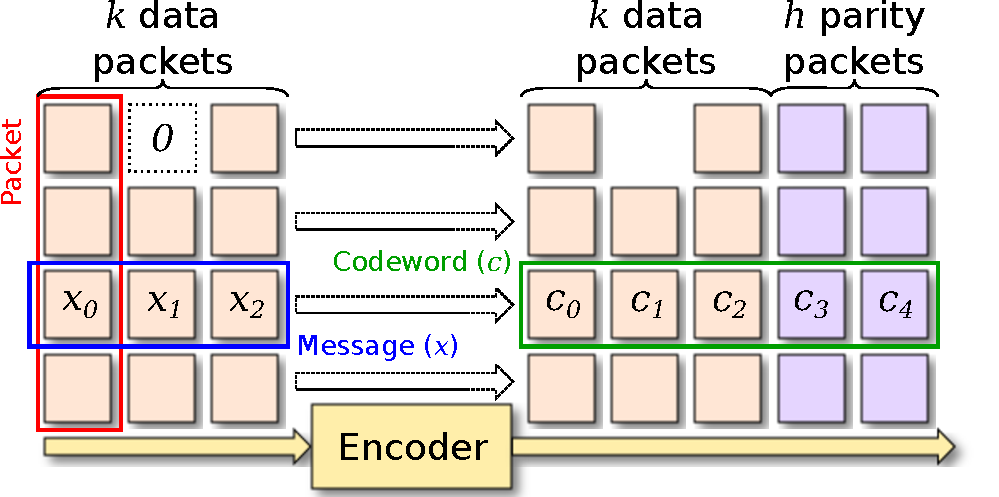
\includegraphics[width=0.4\paperwidth]{Striping.pdf}
  \caption{\label{fig:Striping} Correspondence beween packet data, messages and codewords.
  }
\end{figure}

%In our encoder, the message consists of all symbols in a block that are at a
%certain offset from the start of a data packet.
%Similarly, a codeword contains
%one symbol for each output packet.  We iterate over the offset to generate
%all packets in the block.  If the packet lengths in a group differ, all packets
%will be padded up to the length of the longest packet.
%With the described data assignment, output symbols at
%different offsets are independent, so they can be computed in parallel.  The
%Ethernet MAC produces 64-bit words at a 156.25 Mhz line rate.
%For 8-bit symbols -- corresponding to bytes -- 8 matrix-vector multiplier instances running at
%line rate would suffice to sustain the throughput of the Ethernet MAC.
The encoder could be implemented to work in two ways:
non-incrementally on a group of packets, or incrementally as each
packet arrives. The non-incremental approach is more straightforward,
but incurs high latency and storage requirements, since  encoding
cannot start until all packets in a group have been received.

We opted for the incremental approach, which exploits the associativity of addition to
rearrange the terms of the sums that form the matrix-vector multiplication.
When a new input symbol is received, the partial sums for that symbol are
calculated and the output symbols are updated.

We now derive the resource requirements in terms of multiplications.
The matrix-vector multiplication requires $k \times n$
multiplications. %\FIXME{Not clear what $n$ is}
%\amd{n=k+h ?}
The first $k$ columns are an identity matrix because RSE does not alter data
packets.  The output values can be computed without multiplications.  The
remaining $kh$ multiplications are performed once for each $k$-symbol message,
resulting in $h$ multiplications per input symbol.  As a consequence, we expect that
providing a higher level of protection against erasures for a given throughput
constraint requires more hardware.  The encoder receives
packets from a 10-Gbps Ethernet MAC via a 64-bit AXI bus at a 156.25 Mhz line
rate.  For 8-bit symbols, 8 matrix-vector multiplier instances running at
line rate would suffice to sustain 10 Gbps, so altogether $8h$ Galois-field multiplications
are needed.  To save resources, we use an implementation that computes the
multiplication $m$ of $a$ and $b$ with the formula $m = e^{\log a + \log b}$.
The logarithms and exponents can be looked up in 8-bit tables with 256
entries.
%\amd{8-bit comes out of nowhere.  Do we need to state that we are working
%  with 8-bit symbols (GF(256)?) first for this to make sense?}
Such tables can be implemented in the local memories (BRAMs) of the FPGA.  
The coefficients of the generator matrix are constants.  The associated
logarithms can be precomputed, leaving only 2 lookup tables per multiplier,
resulting in a grand total of $16h$ BRAMs.

Listing~\ref{Multiplier} shows the source code of the
matrix-vector multiplier. %\FIXME{This paragraph+snippet is tricky, since we earlier dismissed using the non-incremental approach.}
It can be compiled with a regular software
compiler and executed on a microprocessor
%, for instance, 
for a software implementation or to debug the code.
In addition, Vivado HLS can generate an FPGA implementation
from the code, guided by the pragmas, which are ignored by software compilers.
A similar implementation in Verilog or VHDL requires in the order of hundreds
of lines.  The {\tt pipeline} pragma directs the tool to construct a
hardware pipeline that can start executing one invocation of the function
every clock cycle.  Vivado automatically inserts a suitable number of registers
to achieve the desired clock period.
The {\tt Par} and {\tt Gen} arrays are mapped
on BRAMs by default.  The pipeline would need {\tt MAX\_H} values from {\tt Par}
per clock cycle although a dual-port BRAM can supply only 2 values.  The
solution is to divide the data in {\tt Par} over multiple BRAMs that can be
accessed simultaneously.  We accomplish that with the {\tt ARRAY\_PARTITION}
pragma.
\hg{Array\_reshape pragma probably makes more sense.  Still have to test it
though.}
\lei{\#Shrink Candidate\#}

\begin{lstlisting}[language=C,basicstyle=\footnotesize,numbers=left,
                   captionpos=b,caption={Matrix-Vector Multiplier},
                   label=Multiplier]
void Enc(char Dat, char Par[MAX_H], int Pkt, int h) {
#pragma HLS ARRAY_PARTITION variable=Par complete dim=1
  static char Gen[MAX_H][MAX_K] = { ... };
#pragma HLS ARRAY_PARTITION variable=Gen complete dim=0
#pragma HLS pipeline
  for (int i = 0; i < MAX_H; i++)
    if (i < h)
      Par[i] = GF_add(Par[i], GF_mul(Dat[j], Gen[i][Pkt]));
}
\end{lstlisting}

% \amd{what do we want to highlight here?
%   (1) data parallel nature of way FEC RSE is defined ... allows operate on
%   the 8 bytes in the 64b per cycle payload independently in data-parallel
%   fashion.
%   (2) as k scales up, demands more compute...which can address with more
%   hardware.
%   (3) result is can build hardware to process in a spatial pipeline at the
%   160\,MHz data rate necessary to meet 10Gbps link.
%   (4) maybe sketch out how much hardware is needed (8$\times$(2+1)$\times$k
%   BRAMs)
% }
% \hg{Ad. 2: I would say h scales up, not k, at least for the encoder.  Are you
% referring to the decoder by any chance?} \amd{yes, I got h and k confused here}

\begin{comment}
Introduce P4.
- Advantages of writing in high-level languages.
- Responsibilities of P4.
- Communication between P4 and encoder
Implementation process
- SDNet
- Vivado HLS
- Vivado
Introduce FPGA.
Top-level design
Matrix multiplication
\end{comment}



\begin{figure}
  \centering
  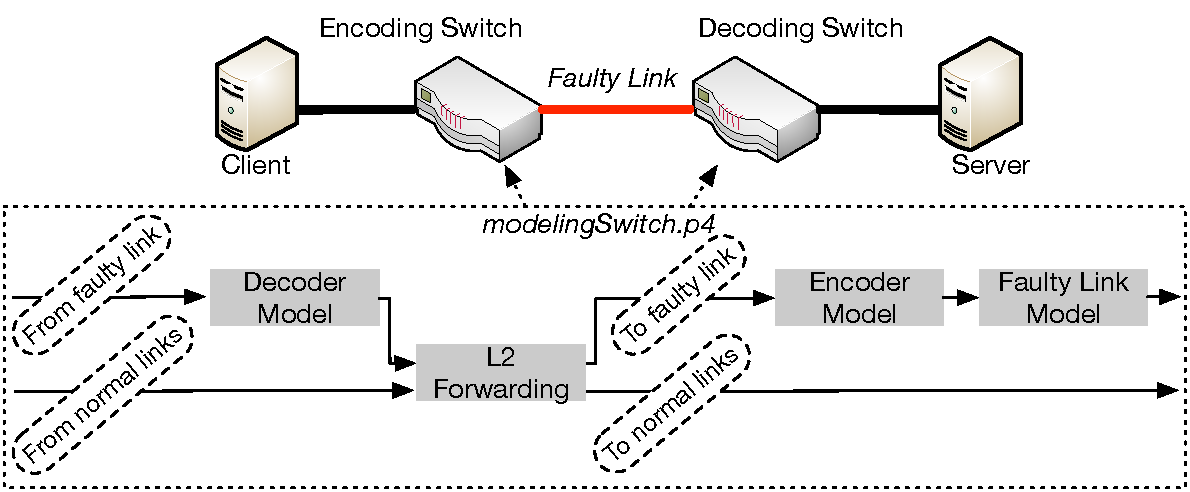
\includegraphics[width=0.40\paperwidth]{figures/lineRateModel.pdf}
  \caption{\label{fig:p4ModelTopo} Topology of the 10 Gb/s testbed 
  for real-time TCP benchmarks, using P4 to model FEC and faulty links.}
\end{figure}

\begin{figure*}[!ht]
\centering
\begin{minipage}[b]{0.31\linewidth}
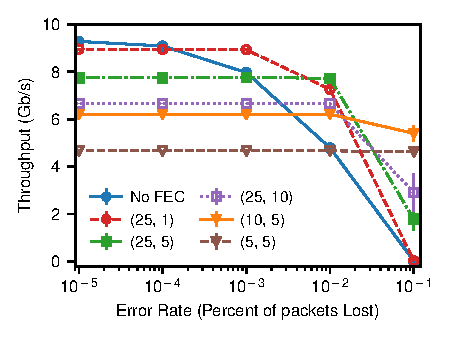
\includegraphics[width=\linewidth]{figures/lossVsTput.pdf}
\caption{Iperf throughput.}
\label{fig:lossVsTput}
\end{minipage}
\hspace{.05in}
\begin{minipage}[b]{0.31\linewidth}
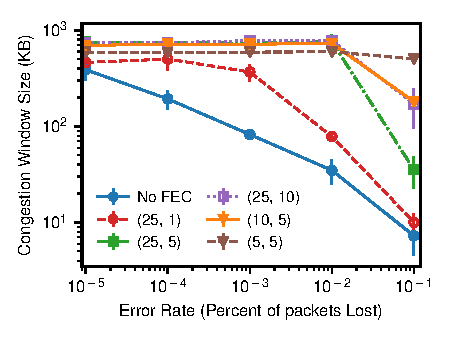
\includegraphics[width=\textwidth]{figures/lossVsWindow.pdf}
\caption{Iperf TCP window sizes.}
\label{fig:lossVsWindow}
\end{minipage}
\hspace{.05in}
\begin{minipage}[b]{0.31\linewidth}
  \centering
  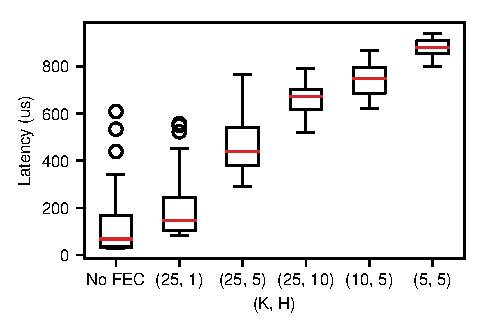
\includegraphics[trim=6mm 6mm 0 0, width=0.95\textwidth]{figures/latency.pdf}
\caption{Latency at error rate=0. Boxes and whiskers show quartile and 1.5*quartile ranges.}
\label{fig:latency}
\end{minipage}
\end{figure*}


\section{Evaluation}
\label{sec:evaluation}
% We evaluate \OurSys using different types of traffic to measure its improvement
% to application-level behavior in the presence of lossy links.

We evaluated \OurSys with microbenchmarks and simulation.
% to answer these questions:
%\begin{itemize}

%\item What are the resource requirements for \OurSys with different levels of 
%error correction?

%\item How much does \OurSys improve application throughput across lossy links?

%\item What benefit can \OurSys have to networks at large?
%\end{itemize}



% We
% evaluate three possible deployment models for \OurSys: an FPGA external to
% the switch; a software implementation running on the switch CPU; and an ASIC  
% implementation integrated into the switch forwarding engine. 

\subsection{\OurSys Models}

\subsubsection{Line Rate P4 Model} 

% \subsection{Setup}
% \begin{figure}
%   \centering
%   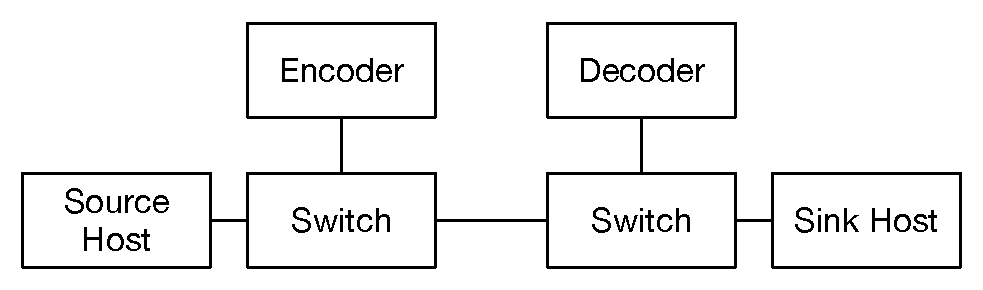
\includegraphics[width=0.3\paperwidth]{exp_topo.pdf}
%   \caption{\label{fig:exp_topo} Testbed topology for benchmarks.}
% \end{figure}

% Figure~\ref{fig:exp_topo} depicts the testbed we used to benchmark \OurSys.
% \hg{This setup was not used to test the FPGA, so it probably does not
% belong in a section on its own.}
% The two traffic generation hosts are each connected to different \OurSys
% enabled switches, which are themselves connected by a 10 GbE link. The
% switches are Wedge BF32-100X's with Barefoot Tofino~\cite{tofino} P4 
% programmable forwarding engines. \lei{TODO: fix cite}


\begin{figure}
  \centering
  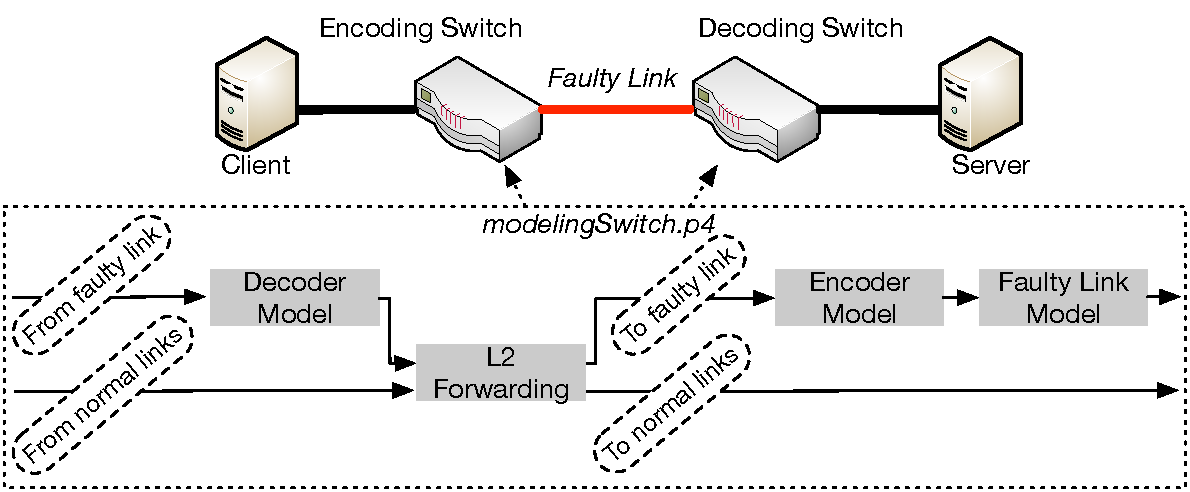
\includegraphics[width=0.4\paperwidth]{figures/lineRateModel.pdf}
  \caption{\label{fig:p4ModelTopo} Topology of the 10 Gb/s testbed 
  network for TCP benchmarks, with line-rate P4 modeling of FEC functionality and faulty links.}
\end{figure}

To measure the effect of faulty links and \OurSys at the application level, we
developed a P4 pipeline for the Barefoot Tofino that models \OurSys. We
deployed the model in a simple 10 Gb/s testbed network, as depicted in
Figure~\ref{fig:p4ModelTopo}, and benchmarked the performance of 
Iperf in real-time. The P4 pipeline models the behavior of the encoder, 
decoder, and faulty link, and can be reconfigured with different FEC and 
packet loss parameters at runtime via the control plane. 

The \textbf{\em encoder model} of the pipeline encapsulates each packet egressing on
the faulty link with the \OurSys header and inserts blank  parity packets into
the flow. It tracks per-port block IDs and  packet indices using P4 register
arrays. To generate parity packets, the  model clones the last data packet in
each block with the Tofino's multicast engine.

The \textbf{\em faulty link model} adds a \emph{corruption header} to each packet
egressing the faulty link. The header indicates whether or not the neighbor
switch should consider the packet lost. The model selects packets for
corruption according to a simple binomial distribution implemented with the
Tofino's random number generator.

Finally, the \textbf{\em decoder model} applies to all packets arriving from a
faulty link, before any other forwarding logic. It removes the corruption
header from each packet and passes non-corrupt packets to the forwarding
pipeline. The model recirculates corrupt packets until the next block begins,
at which point it decides whether they can be recovered based on the number of
non- corrupt data and parity packets it has observed in the block. If it
counted at least K data plus parity packets  in the block, the model
"recovers" all of the corrupt packets by simply removing their corruption
headers and forwarding them normally. If recovery fails, the model drops the
corrupt packets without forwarding.

All experiments we describe below measure performance of 10 second file
transfers from the client to the server, through an encoding switch, faulty
link, and decoding switch. We ran 25 trials for each tested configuration of
K, H,  and loss rate.


\begin{figure*}[!ht]
\centering
\begin{minipage}[b]{0.32\linewidth}
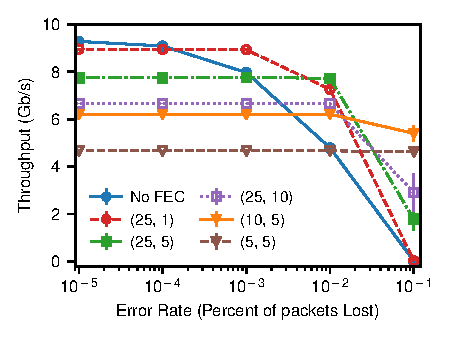
\includegraphics[width=\linewidth]{figures/lossVsTput.pdf}
\caption{Iperf throughput.}
\label{fig:lossVsTput}
\end{minipage}
\hspace{.05in}
\begin{minipage}[b]{0.32\linewidth}
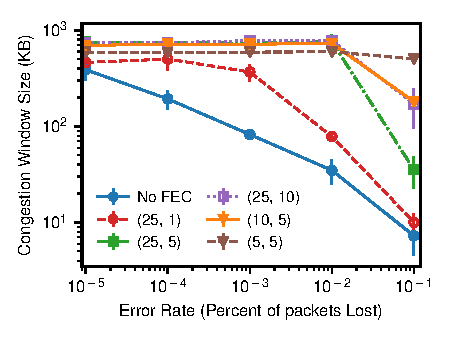
\includegraphics[width=\textwidth]{figures/lossVsWindow.pdf}
\caption{Iperf TCP window sizes.}
\label{fig:lossVsWindow}
\end{minipage}
\hspace{.05in}
\begin{minipage}[b]{0.32\linewidth}
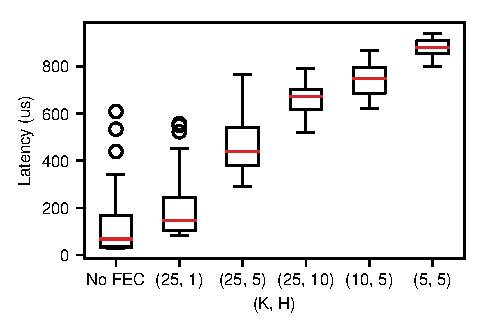
\includegraphics[width=\textwidth]{figures/latency.pdf}
\caption{Network latency.}
\label{fig:latency}
\end{minipage}
\end{figure*}

% \begin{figure}
%   \centering
%   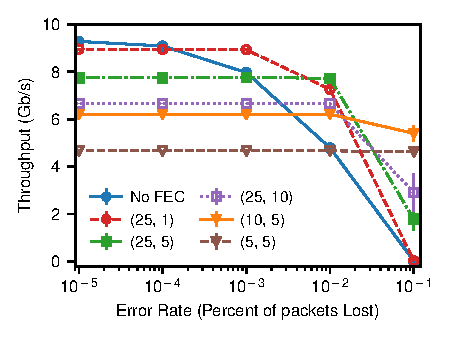
\includegraphics[width=0.3\paperwidth]{figures/lossVsTput.pdf}
%   \caption{\label{fig:lossVsTput} Iperf throughput at different loss rates.}
% \end{figure}

% \begin{figure}
%   \centering
%   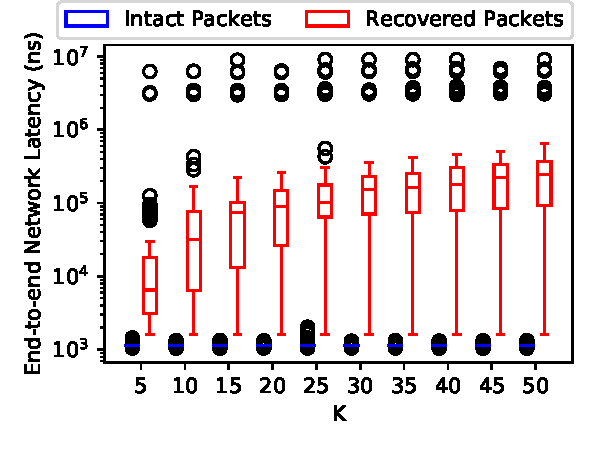
\includegraphics[width=0.3\paperwidth]{figures/udpLatency.pdf}
%   \caption{\label{fig:lossVsLatencyUdp} Network latency for a 100 Mb/s UDP flow (H = 5, loss rate = $10 ^{-2}$).}
% \end{figure}

% \begin{figure}
%   \centering
%   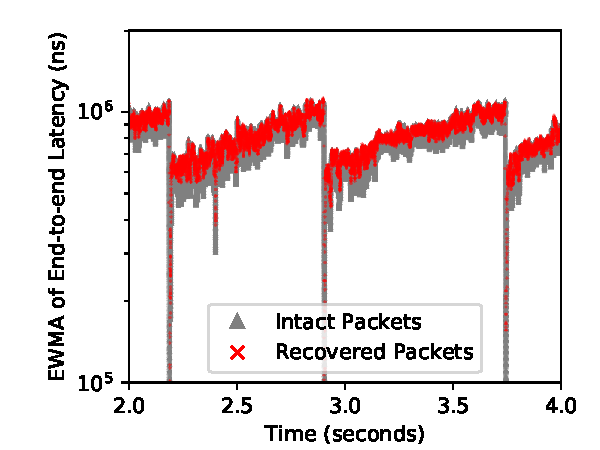
\includegraphics[width=0.3\paperwidth]{figures/tcpLatency.pdf}
%   \caption{\label{fig:lossVsLatencyTcp} Network latency for a 9 Gb/s TCP flow (K = 25, H = 5, loss rate = $10 ^{-2}$).}
% \end{figure}

Figure~\ref{fig:lossVsTput} shows TCP throughput with different FEC
configurations as loss rate varied. With \OurSys, Iperf sustained  over 5 Gb/s
with loss up to $10^{-1}$ (1 out of every 10 packets dropped). Without
\OurSys, Iperf's throughput at that loss rate was under 25 Mb/s. 

Figure~\ref{fig:lossVsWindow} shows average congestion window sizes in 
the trials. Congestion window size ($cwnd$) determines how much data the sender 
can transmit before receiving an ACK, limiting the transmission rate 
to approximately $cwnd$ * round trip time. TCP increases $cwnd$ linearly 
with successful packet deliveries, and reduces it exponentially upon 
packet loss. As Figure~\ref{fig:lossVsWindow} shows, random packet loss 
at rates higher than around $10^{-5}$ causes TCP to reduce $cwnd$ significantly, 
causing the throughput drop in Figure~\ref{fig:lossVsTput}. With FEC, 
the congestion window remains high as loss rate increases, especially when 
using high levels of redundancy, e.g., $(K, H) = (5, 5)$. 

Figure~\ref{fig:latency} shows the in-network latency, i.e., from the  ingress
pipeline of the encoding switch to the egress pipeline of the  decoding
switch, in trials with 0 loss. FEC added under 1 MS of average latency in  all
trials. The amount of latency added by FEC was proportional to $H/K$,  because
the parity packets increased the average length of the egress queue to the
faulty port  by a factor of approximately $H/K$. The additional latency  also
explains why $cwnd$ in Figure~\ref{fig:lossVsWindow} increased with ($H/K$),
as higher latencies require larger window sizes to reach optimal throughput.
\lei{\#Shrink Candidate\#}




% % This figure shows the impact of H. 

% Figure~\ref{fig:lossVsTput} also shows the bandwidth overhead of  FEC, which
% is dominated by the number of parity packets per block ($H$).  At loss rates
% greater than or equal to $10^{-4}$ the bandwidth overhead of adding  parity
% packets had less of an impact on TCP throughput than lost packets, for  most
% configurations tested. To reduce bandwidth overhead, the FEC  can be tuned for the
% loss rate of each specific link, which is reportedly stable over
% time~\cite{corropt}.



% % This figure shows the impact of K.

% To understand how FEC impacts latency, we measured the latency  between the
% ingress pipeline from the source server and the egress pipeline  to the sink
% server, using the nanosecond precision  timestamps of the Tofino, with packets
% routed back through the first  switch before egressing to the sink.
% Figure~\ref{fig:lossVsLatencyUdp}  plots an EWMA of latency for packets in a
% 100 Mb/s UDP flow. For  intact packets, latency was low because they did not
% invoke  the decoder. For  recovered packets, however, the decoder increased
% latency. Average  latency increased with block size because  recovery requires
% the decoder to wait until all the parity packets  for a block arrive. The
% maximum observed latency for recovered packets  was high, around 9 MS. This
% was due to the behavior of the iperf  UDP generator, which periodically paused
% for up to 9 MS between  sending packets, to meet the 100 Mb/s target. The high
% inter-packet  arrival time stalled the generation of parity packets and thus
% the  recovery of any lost packets in the same block.
% \lei{\#Shrink Candidate\#}

% Figure~\ref{fig:lossVsLatencyTcp} plots a time series of latency EWMA  for TCP
% packets in a single maximum rate flow (around 9 Gb/s). The difference in
% latency between recovered versus intact packets was almost indistinguishable.
% Latency for all packets was not dominated by the decoder, but instead by time
% spent  in egress buffers in the switch, which repeatedly filled due to TCPs
% congestion  control dynamics, i.e., causing the familiar ``sawtooth'' pattern
% in Figure~\ref{fig:lossVsLatencyTcp}. Additionally, the latency for packet
% recovery was lower with the TCP workload because average packet rate was
% around 1 order of magnitude higher.







\subsubsection{Event-based simulation}
We customized a fat-tree datacenter topology in ns-3~\cite{ns3-dcn} to
model (i)~a link with loss characteristics as described by Zhuo et
al.~\cite{Zhuo:2017:UMP:3098822.3098849}; and (ii)~FEC to support
transport protocols. In this model we experimented with end-to-end
error correction rather than link-layer, to simulate a more complex
implementation without incurring the burden of implementing it fully.

We simulated a 128-node fat-tree network with 10Gbps links where two
nodes communicate over TCP to transfer a 10MB file at 2Gbps. We found
that using FEC completely eliminated retransmissions (which consisted
  of 152, 23, and 2 packets for loss rates of $10^{-3}$, $10^{-4}$,
and $10^{-5}$ respectively). But achieving end-to-end reliability
over a lossy link with little sacrifice to latency came at a steep
end-to-end overhead of 20\%, since a parity packet was added for each
5 data packets.
Experiments using QUIC suggested that the gains of end-to-end FEC did not
outweigh the bandwidth overhead (even if $h=1$) and adverse affects on video
traffic~\cite[\S7.3]{Langley:2017:QTP:3098822.3098842}.
The approach described in this paper only adds
overhead on lossy links, rather than across paths that contain a
lossy link.


\subsection{Encoder Microbenchmarks}
\iffalse
Here we evaluate the implementation directly, not using a model.
Latency and throughput graphs for experiments involving different loss rates, and the encoder working on the CPU and FPGA.
Note: we have not optimized the CPU implementation.
\fi
We measured the performance of our current encoder implementation.  Packets
in a single flow with uniformly-distributed payload sizes of 64--1450 bytes are
supplied to the FPGA with the packet generator of DPDK 17.08.1. The encoder
processes the packet with parameters $k = 50$ and $h = 1$.
At the output, we measured a throughput of 9.3 Gbps over a 10-minute period,
nearly saturating the 10-Gbps link.

\iffalse
To ensure \OurSys's effect observed in the model are practical, we directly measured the 
full throughput of our encoder implementation in FPGA. For our benchmark, the encoder is configured to use
k=8 and h=4. Packets are generated by a tool based
on DPDK library, and are fed to the board (as is specified above~(\S\ref{sec:implementation})) through
a 10Gbps link. The average outgoing throughput measured during a 10 minutes test is 9.025Gbps.
Considering the overhead from other parts of the system, we believe the link is actually close
to being saturated, which is our basic assumption in evaluations.
\fi

For comparison, we also evaluated a reference CPU implementation, not 
optimized for performance. In the same deployment, its throughput 
measured 227Mbps on a single core, and 1399Mbps using all 8 physical cores of
our Xeon E5-2450L running at 1.8 GHz.

% As a contrast, we also evaluated a CPU implementation, which was not
% optimized for performance, and intended as a reference
% implementation. Under the same deployment, the throughput measured is



\subsection{FPGA resource consumption}
Table~\ref{tab:microbenchmarks} shows the resource requirements for the FPGA implementations of
\OurSys with different $k$ and $h$ parameters.  The resource requirements are
post-implementation utilization values reported by Xilinx Vivado.  We observe
that varying $k$ has a negligible effect on resource consumption, whereas BRAM
consumption has a strong dependence on $h$.  We believe that the BRAM consumption
can be further reduced because several arrays were overpartitioned.
%CPU cycles for the software
%implementation are measured using Linux performance counters and averaged over
%X packets,
%The timing statistics are measured using ingress and egress timestamps on
%the switch.

\begin{table}
% \footnotesize
\begin{center}
\small
% \resizebox{\linewidth}{!}{
\begin{tabular}{ l r r r r } 
\toprule
$(k, h)$ & $(25, 1)$ & $(25, 5)$ & $(25,10)$ & $(50, 1)$ \\
\midrule
%\emph{Software} & & & & \\
%\cmidrule{1-1}
%Cycles & & & & \\
%Proc. Time (ns) & & & & \\
%\midrule
%\emph{FPGA} & & & & \\
%\cmidrule{1-1}
BRAM (18Kb) & 130 (7\%) & 183 (10\%) & 248 (14\%) & 130 (7\%) \\
Flip-flop & 49019 (9\%) & 49291 (9\%) & 49781 (9\%) & 49019 (9\%) \\
LUT & 29909 (11\%) & 30758 (11\%) & 31851 (12\%) & 29919 (11\%) \\
%Proc. Time (ns) & \FIXME{?} & & & \\
\bottomrule
\end{tabular}
% }
\caption{Resource requirement %Comparison
of the FPGA %and CPU
implementation of \OurSys with different configurations.  Note that BRAMs are local memories,
and LUTs (lookup tables) are programmable gates.} % typically implement logic.}
\label{tab:microbenchmarks}
\end{center}
\end{table}

%We run \OurSys in 3 configurations: outside the switch, on the switch, and in the switch.
%Time how quickly \OurSys reacts to failing links.

\section{Conclusion}



\subsection*{Acknowledgements}
This material is based upon work supported by the Defense Advanced
Research Projects Agency (DARPA) under Contracts No. HR001117C0047
and No. HR0011-16-C-0056.
Xilinx provided tools and IP, including SDNet to support P4 to FPGA
compilation, the Ethernet MAC, and HLS and physical design mapping
software. 

\bibliographystyle{ACM-Reference-Format}
\bibliography{paper}

\end{document}
